\documentclass[tikz,border=2]{standalone}
\usetikzlibrary{shadows,arrows,shapes,positioning,calc,backgrounds,fit,automata}
\usetikzlibrary{decorations.text}
\usepackage{varwidth}
\usepackage[scaled]{libertine}
%%\usepackage[scaled]{helvet}
\renewcommand{\familydefault}{\sfdefault} 
%% \usepackage{lmodern} % enhanced version of computer modern
\usepackage[T1]{fontenc} % for hyphenated characters and textsc in section title
\usepackage{amssymb}
\usepackage{mathtools} % contains amsmath which comes with align
\usepackage{amsthm}
\usepackage{graphicx}
\graphicspath{{aux/}}
\usepackage{microtype} % some compression
\usepackage[skins]{tcolorbox}
\begin{document}
%%%%%%%%%%%%%%%%%%%%%%%%%%%%%%%%%%%%%%%
% Define the layers to draw the diagram
\pgfdeclarelayer{bg}
\pgfsetlayers{bg,main}
%%%%%%%%%%%%%%%%%%%%%%%%%%%%%%%%%%%%%%%
% colors
\definecolor{DarkRed}{HTML}{D8392B}
\definecolor{DarkBlue}{HTML}{558B92}
\definecolor{DarkBrown}{HTML}{62524F}
\definecolor{DarkGreen}{HTML}{A18F6A}
\definecolor{Red}{HTML}{E65942}
\definecolor{Blue}{HTML}{78A4AC}
\definecolor{Brown}{HTML}{7B6663}
\definecolor{Green}{HTML}{C4AE87}
\definecolor{Grey}{HTML}{D3D3D3}
%%%%%%%%%%%%%%%%%%%%%%%%%%%%%%%%%%%%%%%
% wheel chart stuff
%%%%%%%%%%%%%%%%%%%%%%%%%%%%%%%%%%%%%%%
% Adjusts the size of the wheel:
\newcommand{\ring}[5]{
\def\outerradius{#2}
\def\innerradius{#3}
\pgfmathsetmacro{\cumnum}{#4}
\pgfmathsetmacro{\totalangle}{#5}
\def\segmentgapfraction{5}

\pgfmathsetmacro{\totalnum}{0}
% Calculate the thickness and the middle line of the wheel
\pgfmathsetmacro{\midradius}{(\outerradius+\innerradius)/2}

\foreach \value/\colour/\name/\label in {#1} {
    \pgfmathparse{\value+\totalnum}
    \global\let\totalnum=\pgfmathresult}

% Loop through each value set. \cumnum keeps track of where we are in the wheel
\foreach \value/\colour/\name/\label in {#1} {
    \pgfmathsetmacro{\newcumnum}{\cumnum + \value/\totalnum*\totalangle}
    \pgfmathsetmacro{\truncnewcumnum}{\newcumnum-\segmentgapfraction}
    
    % Calculate the mid angle of the colour segments to place the labels
    \pgfmathsetmacro{\midangle}{-(\cumnum+\newcumnum)/2}
    
    % This is necessary for the labels to align nicely
    \pgfmathparse{(\cumnum>90?1:0)} \edef\westind{\pgfmathresult}
    \pgfmathparse{(\cumnum<270?(\westind*1):0)} \edef\westind{\pgfmathresult}
    \pgfmathparse{((\westind==1)?"east":"west")} \edef\textanchor{\pgfmathresult}
    \pgfmathsetmacro{\labelshiftdir}{1-2*(\westind)}
    
    % Draw the color segments. Somehow, the \midrow units got lost, so we add 'pt' at the end. Not nice...
    \fill[\colour,opacity=1] (\cumnum:\outerradius) arc (\cumnum:\truncnewcumnum:\outerradius) 
        -- (\truncnewcumnum:\innerradius) arc (\truncnewcumnum:\cumnum:\innerradius) 
        -- cycle;
    
    % Draw the data labels
        \draw  [\colour,thin,text=black] node [append after command={(\cumnum:\innerradius)
    -- (\cumnum:\outerradius + 2ex) 
    -- (\tikzlastnode.\textanchor)}] at
    (\cumnum:\outerradius + 2ex) [xshift=\labelshiftdir*.2cm,
anchor=\textanchor,text=DarkBrown]{\small \name};
    
    % Set the old cumulated angle to the new value
    \global\let\cumnum=\newcumnum
}
}

\newcommand{\circtext}[7]{
\def\outerradius{#2}
\def\innerradius{#3}
\def\midradius{#4}
\pgfmathsetmacro{\cumnum}{#5}
\pgfmathsetmacro{\totalangle}{#6}
\pgfmathsetmacro{\opacity}{#7}
\def\segmentgapfraction{5}

\pgfmathsetmacro{\totalnum}{0}
% Calculate the thickness and the middle line of the wheel
%%\pgfmathsetmacro{\midradius}{\outerradius/2+\innerradius/2}

\foreach \value/\colour/\name/\textcolor in {#1} {
    \pgfmathparse{\value+\totalnum}
    \global\let\totalnum=\pgfmathresult}

% Loop through each value set. \cumnum keeps track of where we are in the wheel
\foreach \value/\colour/\name/\textcolor in {#1} {
    \pgfmathsetmacro{\newcumnum}{\cumnum + \value/\totalnum*\totalangle}
    \pgfmathsetmacro{\truncnewcumnum}{\newcumnum-\segmentgapfraction}
    
    % Calculate the mid angle of the colour segments to place the labels
    \pgfmathsetmacro{\midangle}{-(\cumnum+\newcumnum)/2}
    
    % This is necessary for the labels to align nicely
    \pgfmathparse{(\cumnum>90?\cumnum:\truncnewcumnum)} \edef\startangle{\pgfmathresult}
    \pgfmathparse{(\cumnum>90?\truncnewcumnum:\cumnum)} \edef\endangle{\pgfmathresult}
    
    % Draw the color segments. Somehow, the \midrow units got lost, so we add 'pt' at the end. Not nice...
    \fill[\colour,opacity=\opacity,thick] (\cumnum:\outerradius) arc (\cumnum:\truncnewcumnum:\outerradius) 
        -- (\truncnewcumnum:\innerradius) arc (\truncnewcumnum:\cumnum:\innerradius) 
        -- cycle;
    
    % Draw the data labels
        \draw [draw=none, font=\small,thick,postaction={decorate,decoration={text along path,text
        align=center,text color=\textcolor,text={\name}}}] (\startangle:(\midradius) arc
    (\startangle:\endangle:\midradius);

    
    % Set the old cumulated angle to the new value
    \global\let\cumnum=\newcumnum
}
}

\begin{tikzpicture}
    \node [inner sep=0,minimum size=4.8cm,text=DarkBrown] at (0.2,.5)
    {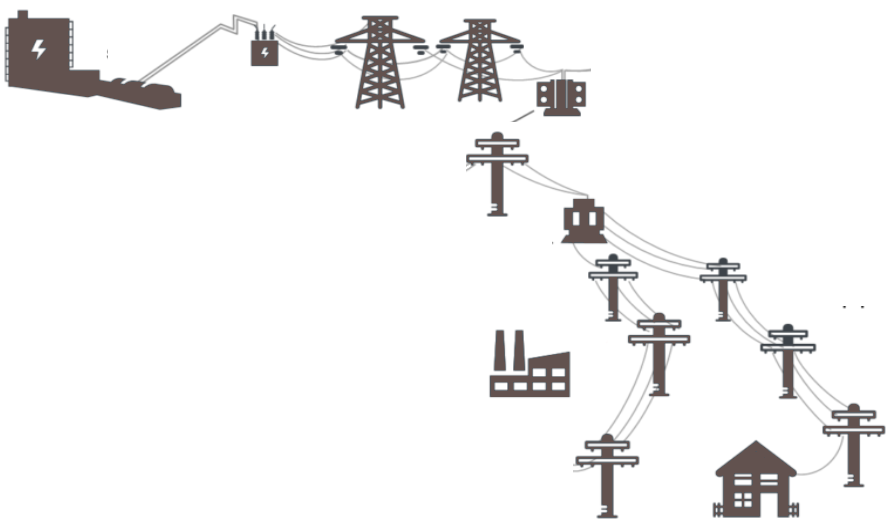
\includegraphics[width=5.5cm,trim={0cm 0cm 0cm 0cm},clip]{power_network_v2.png}};
    \node [circle,inner sep=-1pt,text=Red,draw=Brown,thin] at (-1.2,-.2)
    {\parbox{2.5cm}{\centering\large\textsc{State}\\\textsc{Estimation}\\
      \small $\mathbf{z}=\mathbf{h}(\mathbf{x})+\mathbf{e}$}};
%%%%%%%%%%%%%%%%%%%%%%%%%%%%%%%%%%%%%%%%%%%%%%%%%%%%%%%%%%%%%%%%%%%%%%%%%%%
% data
%%%%%%%%%%%%%%%%%%%%%%%%%%%%%%%%%%%%%%%%%%%%%%%%%%%%%%%%%%%%%%%%%%%%%%%%%%%
    \ring{
        1/Brown/\parbox{1.6cm}{Power grid topology}/, 
        1/Brown/PMU/,
        1/Blue/\parbox{1.3cm}{Demand model}/,
        1/Blue/\parbox{1cm}{Smart
        meters}\raisebox{-.3cm}{
\includegraphics[width=.75cm]{smart_meter.png}}/, 
        1/Blue/\parbox{1.1cm}{Market
        prices}\raisebox{-.2cm}{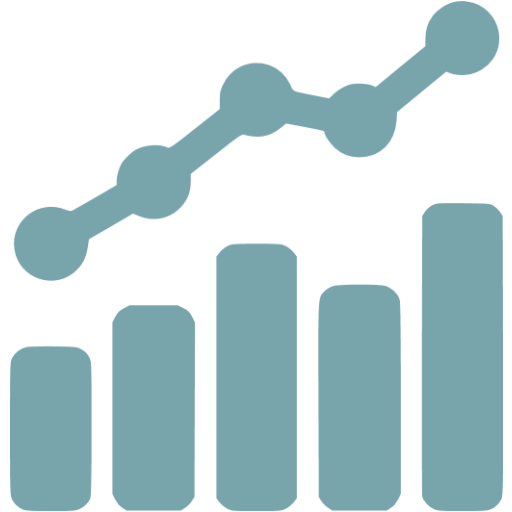
\includegraphics[width=.75cm]{market_prices.png}}/, 
        1/Green/\parbox{1cm}{LiDAR}\raisebox{-.4cm}{
\includegraphics[width=1.2cm]{lidar_icon.png}}/, 
        1/Green/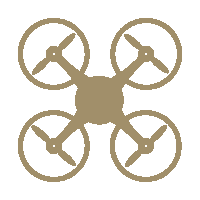
\includegraphics[width=.7cm]{drone_icon_green.png}\raisebox{.1cm}{\parbox{5cm}{Optical cameras using drones}}/, 
    1/Green/Thermal camera/}{4cm}{3.9cm}{150}{160} 
    \circtext{2/Brown/Direct/Brown, 3/Blue/Social/Brown, 3/Green/Imagery/Brown}
    {3.8cm}{3.35cm}{3.7cm}{150}{160}{.2}
    \circtext{1/Red/Data and measurements/white}
    {3.3cm}{2.9cm}{3.2cm}{150}{160}{1}
%%%%%%%%%%%%%%%%%%%%%%%%%%%%%%%%%%%%%%%%%%%%%%%%%%%%%%%%%%%%%%%%%%%%%%%%%%%
% methods
%%%%%%%%%%%%%%%%%%%%%%%%%%%%%%%%%%%%%%%%%%%%%%%%%%%%%%%%%%%%%%%%%%%%%%%%%%%
    \ring{
        1/Brown/Transfer learning/, 
        1/Brown/Neural networks/,
        1/Brown/CART/,
        1/Blue/\parbox{2cm}{Approximation algorithms}/,
        1/Blue/\parbox{1.7cm}{Distributed algorithms}/,
        1/Green/\parbox{2.3cm}{Parametric \& non-parametric inference}/
    }{3.7cm}{3.6cm}{310}{120}
    \circtext{1/Brown/Methods/white}
    {3.5cm}{3.05cm}{3.4cm}{310}{120}{1}
%%%%%%%%%%%%%%%%%%%%%%%%%%%%%%%%%%%%%%%%%%%%%%%%%%%%%%%%%%%%%%%%%%%%%%%%%%%
% Problems
%%%%%%%%%%%%%%%%%%%%%%%%%%%%%%%%%%%%%%%%%%%%%%%%%%%%%%%%%%%%%%%%%%%%%%%%%%%
    \ring{
        1/Brown/Data fusion/, 
        1/Blue/Resource constrained sensing/,
        1/Green/\parbox{2.5cm}{State estimation after WMD attacks}/,
        1/Grey!80/\parbox{2.2cm}{Computational efficiency}/
    }{4.1cm}{4cm}{70}{80}
    \circtext{1/Green/Problem space/white}
    {3.9cm}{3.45cm}{3.6cm}{70}{80}{1}
\end{tikzpicture}
\end{document}
